\chapter{History and recent advancements}
\label{kap:kap1}

The size of information and data grows exponentially over years. In order to store this data, we use different data structures. These data structures not only represent the data but also enable us to make certain operations over them. There is a significant effort in not only speeding up these structures but also making them smaller in size so that they can be managed in memory and not on a secondary data storage thas is often orders of magnitude time slower. The key factor is to find the right balance between the speed of common operations and the amount of information that we need to store.

\section{Space-efficient data structures}

When we measure how space-efficient the data structure is, we often measure this in additional information that we store alongside the original data. Most of the time, with the complexity of operations that our data structure supports, the size of metadata stored also increases. The original data can be however also compressed to further increase the space-efficiency. To remove ambiguity, we measure the size of the original data as the information-theoretical optimal number of bits used to store the original data. We will now introduce the basic definition that distinguishes between space-efficiency of data structures:

Let's say that X is the information-theoretical optimal number of bits needed to store the data. A data structure representing this data is called:
\begin{itemize}
\item implicit if it takes $X + O(1)$ bits of space
\item succinct if it takes $X + O(X)$ bits of space
\item compact if it takes $O(X)$ bits of space
\end{itemize}

As an example, the common representation of string in a language such as C uses the null-termination method. In this form, the original string is stored in memory with the null termination character just after the end of the string. It is easy to see that this representation is implicit. To represent the string we could also store the string and only remember it's length, not using the null termination character. This would, however, lead to a succinct data structure as we need $O(log(X))$ bits to store the length of the string.

The amount of data that these types of structures are dealing with is many times too big to store linear number of additional data for our operations so a lot of the solutions in this area aim for a sublinear number of additional data.

It should be clear that the additional requirement on the data structure to be space-efficient many times leads to worse time complexity. Even if the theoretical time complexity remains the same for compressed data structures, the real-world implementation can suffer in performance as the methods that are used for work with compressed data are many times not ideal in the classical computer model.

\subsection{K-th order entropy}

\begin{theorem}
Let's have a string $S$ with size $n$ and $n_i$ denoting number of occurences of character
on position $i$. Empirical entropy of string $S$ is denoted $H_0(S)$ and defined as:
\begin{center}
$H_0(S) = \frac{1}{n} \sum_{i=1}^{k} n_i\cdot log(\frac{n}{n_i})$
\end{center}
\end{theorem}

Most of these algorithms use as a measure of information stored a $k$-order empirical entropy.

\begin{theorem}
Let's have a string $S$ and construct $S_w$ as a string obtained by concatenating the characters immidiately following occurences of $w$ in $S$.
$k$-order empirical entropy ($k \geq 1$) of $S$ denoted $H_k(S)$ is defined as:
\begin{center}
$H_k(S) = \frac{1}{n} \sum_{|w|=k} |S_w| H_0(S_w)$
\end{center}
\end{theorem}

This is a measure of information that is emitted with respect to the previous $k$-characters. This type of a model is especially useful when we know
that we are dealing with some data that can be thought of as generated using the Markov process.

\section{History and recent progress in the field}

We will now look briefly into the history and then on recent results in this topic. The field dates back to the Jacobsen work on static succinct data structures. Jacobsen distinquishes between data compression, when we take the big chunk of data and try to fit it into a smaller place and
data optimization when we want to actively do queries over this stored information. His work mainly looked into space-efficient representation of linked lists, trees and direct-acyclic graphs with traversing operations over them.

There are of course many possible data structures and operations that they can support in order to be reasonable to use. We will now look at the most common operations that are supported in the succinct data structures. Surprisingly, from our observations they are not that diverse.

\begin{theorem}
Let's say that we have a finite sequence of $N$ elements.
We define two operations rank and select: \\
$rank_q(x) = | \{ k \in [ 1, 2, \ldots, x]:N[k] = q  \} |$ \\
$select_q(x) = min \{ k \in [ 1, 2, \ldots, n):rank_q(k)=x  \} $
\end{theorem}

In other words, $rank_q(x)$ denotes the number of elements in $N$ that are equal to $q$ and their position in $N$ is less than $x$. $select_q(x)$ returns the position of $x$-th occurence of $q$.
These two types of operations are very common in succinct data structures. Let's say we want to store the sequence of elements that are not of fixed size.
With the sequence of data, represented by the individual bits of elements. We can also store metadata in the form of bit-vector, that has one's on the indexes
where the new element begins as we see in Fig. \ref{obr:obr_rank_select}.

\begin{figure}
\centerline{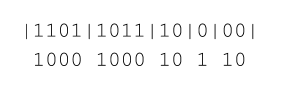
\includegraphics[width=0.4\textwidth]{images/obr_rank_select}}
\caption[Rank select usage in representation of sequence of elements with different size]{Rank select used in metadata, denoting start of the element.}
\label{obr:obr_rank_select}
\end{figure}

\subsection{RRR}

RRR is used for representing static bitmaps. We split the binary representation of data into big chunks, which we call blocks.
Each $f$ of subsequent blocks are connected into non-overlapping superblocks. Each block is then encoded as a pair of integers $(c, o)$. $c$
is the count of the set bits in the corresponding block and $o$ is an offset into the table $T[c]$ that stores in lexicographic order all the sequences of
length $b$ with $c$ bits set to 1. There are two types of what the word dynamic means. Let's say that our data structure represents some sequence of numbers.
In some cases, it can refer to the ability to change some value in the underlying sequence. In other cases, it refers to the possibility to insert a new element at the arbitrary
position in the sequence.

\subsection{Run length encoding}

Another widely used type of storage is run length encoding. We will assume, that one of the values in bit-vector(either 0 or 1) is more frequent than the other. Let's say that we know, there are way more zeroes present in our data. It is natural to expect that there will be a lot of subsequent occurences of zeroes that we call runs. We will store only the lengths of zero runs between the subsequent ones. So for example
sequence $0001011001000$ is stored as $3, 1, 0, 2, 3$.

 We can now compress subsequent runs of zeroes and write them as the index $0^{p_1}10^{p_2}110^{p_3}\ldots 10^{p_k}$. 

\section{Dynamic succinct data structures}

The most recent results in succinct data structures look into how to make these data structures more usable in real-life scenarios. Many times, the
strongest assumption of these data structures is, that the data we store is not changing in any way. For a few years now, there is a considerable amount
of effort put into dynamic succinct data structures. 

\subsection{Searchable Partial Sums with Inserts}

\begin{theorem}
The Searchable Partial Sums with Inserts (SPSI) problem is a problem, requiring the data structure to
store sequence $x_1, x_2, \ldots , x_n$ of non-negative $l$-bits integers and supporting the opperations:
\begin{itemize}
    \item $sum(i) = \Sigma_{j=1}^{i} x_j$
    \item $search(s) = min(\{i : \Sigma_{j=1}{i} x_j > s \})$
    \item $update(i, k): \forall k \in Z, k \geq 0 \lor (k\leq 0 \implies x_i + k \geq 0): x_i \rightarrow x_i + k$
    \item $insert(i): x_1, x_2,\ldots, x_n \rightarrow x_1, x_2,\ldots , x_{i-1}, 0, x_{i}, \ldots , x_n$
\end{itemize}
\end{theorem}

This problem is also very popular in relation to succinct data structures. It is because of his close relationship with the bit-vectors.
As can be seen in [Dynamic], this data structure can be used to represent the bit-vector. In real implementations, the data structure
implementing these operations can be efficiently implemented using the B-tree.
